
\documentclass[sigconf,anonymous,review]{acmart}
\acmSubmissionID{1570}

\usepackage{booktabs} % For formal tables
\usepackage{color}
 % to balance the end of two columns
\usepackage{balance}
\usepackage{bm}
% TOG prefers author-name bib system with square brackets
%\citestyle{acmauthoryear}
%\setcitestyle{nosort,square} % nosort to allow for manual chronological ordering



\usepackage[ruled]{algorithm2e} % For algorithms
\renewcommand{\algorithmcfname}{ALGORITHM}
\SetAlFnt{\small}
\SetAlCapFnt{\small}
\SetAlCapNameFnt{\small}
\SetAlCapHSkip{0pt}

% Metadata Information
%\acmJournal{TOG}
%\acmVolume{38}
%\acmNumber{4}
%\acmArticle{39}
%\acmYear{2019}
%\acmMonth{7}

% Copyright
%\setcopyright{acmcopyright}
%\setcopyright{acmlicensed}
%\setcopyright{rightsretained}
%\setcopyright{usgov}
%\setcopyright{usgovmixed}
%\setcopyright{cagov}
%\setcopyright{cagovmixed}

% DOI
%\acmDOI{0000001.0000001_2}

% Paper history
%\received{February 2007}
%\received{March 2009}
%\received[final version]{June 2009}
%\received[accepted]{July 2009}

\setcopyright{acmcopyright}
\copyrightyear{2020}
\acmYear{2020}
\acmDOI{10.1145/1122445.1122456}

%% These commands are for a PROCEEDINGS abstract or paper.
\acmConference[MM '20]{Proceedings of the 27th ACM International Conference on Multimedia}{October 21--25, 2020}{Seattle, US}
\acmBooktitle{Proceedings of the 27th ACM International Conference on Multimedia (MM '20), October 21--25, 2020, Seattle, US}
\acmPrice{15.00}
\acmISBN{978-1-4503-XXXX-X/20/06}

\newcommand{\cxj}[1]{\textcolor{red}{(#1)}}
\newcommand{\td}[1]{\textcolor{blue}{#1}}
\newcommand{\rmv}[1]{\textcolor{green}{#1}}
\newcommand{\real}{{\mathbb{R}}}
\newcommand{\synS}{\mathcal{S}_{syn}}
\newcommand{\dfmS}{\mathcal{S}_{dfm}}
\newcommand{\hdS}{\mathcal{S}}
\newcommand{\dlt}[1]{}


% Document starts
\begin{document}
% Title portion
%\title{FaceSketching: Interactive Realistic Face Image Creation from Free-hand Sketches }
\title{DeepFacePencil: Creating Face Images from Freehand Sketches}

\begin{abstract}
In this paper, we explore the task of generating photo-realistic face images from hand-drawn sketches. 
%
Existing image-to-image translation methods require a large-scale dataset of paired sketches and images for supervision.
They typically utilize synthesized edge maps of face images as training data. 
However, these synthesized edge maps strictly align with the edges of the corresponding face images, which limit their generalization ability to real hand-drawn sketches with vast stroke diversity. 
To address this problem, we propose DeepFacePencil, an effective tool that is able to generate photo-realistic face images from hand-drawn sketches, based on a novel dual generator image translation network during training. 
%
A novel spatial attention pooling (SAP) is designed to adaptively handle stroke distortions which are spatially varying to support various stroke styles and different level of details.
We conduct extensive experiments and the results demonstrate the superiority of our model over existing methods on both image quality and model generalization to handdrawn sketches.
\end{abstract}

% The code below should be generated by the tool at
% http://dl.acm.org/ccs.cfm
% Please copy and paste the code instead of the example below.
%
\begin{CCSXML}
	<ccs2012>
	<concept>
	<concept_id>10010147.10010257.10010293.10010294</concept_id>
	<concept_desc>Computing methodologies~Neural networks</concept_desc>
	<concept_significance>500</concept_significance>
	</concept>
	</ccs2012>
\end{CCSXML}

\ccsdesc[500]{Computing methodologies~Neural networks}

%\keywords{spatial attention; conditional generative adversarial nets; face; sketch; realistic images}

%
% End generated code
%


\keywords{Image synthesis, spatial attention, sketch-based interface,
face editing, conditional generative adversarial networks}

\dlt{
\begin{teaserfigure}
	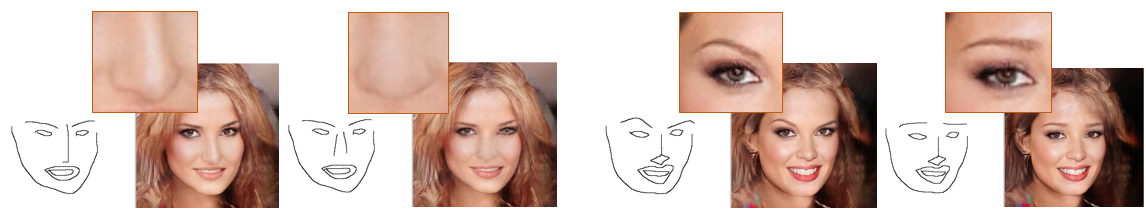
\includegraphics[width=\textwidth]{figs/teaser.png}
	\caption{This is a teaser}
	\label{fig:teaser}
\end{teaserfigure}
}

\maketitle

% !TeX root = ../main.tex

\chapter{绪论}

\section{研究背景}

%\subsection{二级节标题}
%
%\subsubsection{三级节标题}
%
%\paragraph{四级节标题}
%
%\subparagraph{五级节标题}

人脸图像生成一直是计算机图形和视觉领域的热门方向,包括人脸姿态仿真\cite{Yin_2017_ICCV}、遮挡人脸恢复\cite{Li_2017_CVPR}、年龄与表情仿真\cite{G_2017_ICIP,ggfr}、面部属性编辑\cite{attrgan}、人脸艺术生成\cite{carigan}、人脸美颜与风格化\cite{beautygan}等等。而基于草图的人脸图像生成是这一方向的重要分支。

当我们想要从零开始描绘一个物体时,手绘草图无疑是最直观、最有效的方式之一,它比文字描述更清晰具象,可以将抽象的概念转化为具体的视觉表达。随着触屏设备的广泛普及,随手绘制草图变得越来越简单容易。所以如何由手绘草图生成真实的图像一直吸引着领域内研究人员的关注。由手绘草图生成真实的人脸有着广泛的应用。比如在刑侦案件中,根据目击者的手绘草图重塑嫌疑人的人脸图像;还可以根据我们自己的兴趣,随心所欲地将手绘的人脸草图转化成真实的人脸照片等等。而且,草图有着很强的通用性,是一种跨越国家和文化的沟通交流方式,不同国家和民族的人们都可以通过手绘草图描绘自己的所见所闻,表达自己的所思所想。草图简单明了,但却可以捕捉对象的结构特征和纹理细节,包含了足够的信息,可以作为有效的输入来生成高质量的图像。

经过近二十年的发展,由草图生成真实图像的方案主要有两种。一种是传统的方法,图像检索。该方法需要基于一个庞大的数据库,将手绘草图分割成独立的部分,利用搜索算法分别检索出与输入的草图相匹配的图像,然后将所有部分进行融合,生成一张完整的图像。该方法缺点很明显,那就是需要大量的数据,保证数据库中有与输入草图相匹配的内容,并且后期的融合会有很明显的痕迹。这种方法显然不适合人脸图像的生成。

另一种是基于深度学习的方法,图像翻译\cite{pix2pix}。图像翻译的目标是给定输入-输出图像对作为训练数据,将输入图像从一个域$\mathscr{A}$(源域)转换到另一个域$\mathscr{B}$(目标域)。如果用$\alpha (x, \symup{A}) \in \mathscr{A}$和$\beta(x,\symup{B})\in\mathscr{B}$来表示域$\mathscr{A}$和域$\mathscr{B}$的图像,图像翻译的任务可以描述为,寻找一个合适的变换$f:\mathscr{A}\to\mathscr{B}$,使得
\begin{equation}
  f(\alpha (x, \symup{A})) = \beta(x,\symup{B})
\end{equation}

该方法基于生成对抗网络GAN\cite{gan},并且是以图像为输入的条件生成对抗网络\cite{cgan}。在训练阶段,需要大量成对的数据作有监督的学习。条件生成对抗网络的网络结构分为两部分,即生成器和判别器。训练时将草图输入生成器,生成一张图像,然后将生成的图像与真实的图像分别输入判别器,以判别器的输出代入损失函数,分别计算生成器与判别器的损失,通过后向传播算法更新网络参数,使生成器产生更接近真实图像的输出。图像翻译的概念最早由朱俊彦在pix2pix\cite{pix2pix}这篇论文中提出,而后又在此基础上发表了另一篇文章pix2pixHD\cite{pix2pixhd},可以生成质量更高的图像。本文的主要工作就是围绕pix2pixHD展开。

\section{本文工作}

本文旨在探究利用pix2pixHD实现从草图到人脸照片生成的过程,发现对于手绘草图的输入,其输出结果的质量不够令人满意,特别是某些细节比较模糊,而且草图上某一位置的改变常引起生成结果全局的变化。针对这一缺陷,我们用可视化的手段分析了草图特征,对其网络结构进行了深度剖析,在此基础上改造了其生成器的网络结构,我们改进后的模型对手绘草图输入的生成图像质量更高,并且能更好地实现图像编辑的功能。

首先,本文用人脸轮廓-照片数据对训练pix2pixHD的原始模型,然后用手绘的草图进行测试,发现其生成的人脸照片不尽人意,具体表现为纹理特征不够清晰,丧失了对细节的控制,如果在草图上改动一处可能影响生成的整体结果。

而后,利用pca、tsne等可视化工具对生成器网络提取到的草图特征进行可视化分析,结合对网络结构的研究,本文发现生成器编码图片所用的实例标准化层是造成这一现象的根本原因。接下来我们针对生成器中的实例标准化层进行了消融实验,做对比研究,发现去掉前两层实例标准化操作的模型生成质量更高,且能更好地对输入草图进行编辑。

针对模型对于输入草图空间位置变化的鲁棒性差的问题,我们用增广的数据重新训练了模型,成功解决了这一问题。

%\section{脚注}
%
%Lorem ipsum dolor sit amet, consectetur adipiscing elit, sed do eiusmod tempor
%incididunt ut labore et dolore magna aliqua.
%\footnote{Ut enim ad minim veniam, quis nostrud exercitation ullamco laboris
%  nisi ut aliquip ex ea commodo consequat.
%  Duis aute irure dolor in reprehenderit in voluptate velit esse cillum dolore
%  eu fugiat nulla pariatur.}

\section{Related Work}

\subsection{Image-to-Image Translation}
Given an input image from one domain, an image-to-image translation model outputs a corresponding image from another domain and preserves the content in the input image. Existing image-to-image translation models are based on generative adversarial networks conditioned on images. 
%
Pix2pix~\cite{pix2pix} is the first general image-to-image translation model which is able to be applied to different scenarios according to the paired training images, such as, semantic maps to real images, day images to night images, image coloring, and edge maps to real images. 
%
\cite{outdoor_scene} utilizes semantic label maps and attributes of outdoor scenes as input and generates the corresponding photo-realistic images.
%
In order to model multi-modal distribution of output images, BicycleGAN~\cite{BicycleGAN} encourages the connection between the output and the latent code to be invertible.
%
CycleGAN~\cite{CycleGAN}, DualGAN~\cite{DualGAN}, and DiscoGAN~\cite{DiscoGAN} propose unsupervised image translation model with a similar idea named cycle consistency borrowed from language translation literature. 
%
StarGAN~\cite{StarGAN} presents a framework for one-to-many image translation by adding a domain code as input and a domain classifier as guidance.
%
Pix2pixHD~\cite{pix2pixHD} is proposed as a high-resolution image-to-image translation model for generating photo-realistic image from semantic label maps using a coarse-to-fine generator and a multi-scale discriminator. It can also be applied to edge-to-photo generation by using the paired edge maps and photos as training data.
%
\td{However, xxxxxxxxxxxxxx}

\subsection{Sketch-based Image generation}
Sketch-based image generation is a hot topic in computer vision and computer graphics. Given a sketch of a scene with text labels for objects, traditional methods, such as Sketch2Photo~\cite{Sketch2Photo} and PhotoSketcher~\cite{PhotoSketcher}, search corresponding image patches from a large image dataset and then fuse the the retrieved image patches together according to the sketch. These methods are not able to ensure the global consistency of the resultant image and fails to generate totally new images.
%
After the breakthrough made by deep neural networks (DNN) in computer graphics and computer vision, a variety of DNN-based models have been proposed for sketch-based image generation. 
%
The general image-to-image translation models mentioned above are able to be applied to sketch-based image generation once sketches and the corresponding images are used as training data.
%
Besides, many other models are designed specially for sketch inputs. SketchyGAN~\cite{SketchyGAN} aims to generate real images from multi-class sketches. A novel neural network module, called mask residual unit (MRU), is proposed to improve the information flow by injecting the input image at multiple scales. \td{Edge maps are extracted from real images and utiled as training sketches.} However, the resultant images of SketchyGAN are still not satisfied.
%

\subsection{pooling}

\subsection{Face Generation and Editing}

\td{All existing methods for local face editing require the user to provide masks and strokes manually}. In comparison, strokes are only the input to indicate the desired shape. Our system automatically interprets the intended edit and produces the local change accurately. This greatly reduces users' burden and preserves the fluency of user interaction. 

\td{Only local edit in a relatively small area is supported.} As reported in SC-FEGAN~\cite{}, artifacts appear when complete a large region in FaceShop~\cite{}.

\section{Deep Network for Sketch-Photo Translation}
\label{sec:network}

\subsection{Edge alignment in baseline Model}

Generating a realistic photo from sketch can be considered as an image translation problem. 
We use the state-of-the-art Pix2PixHd~\cite{} as our baseline. 
% 
 
We use the CelebA-HD dataset~\cite{} which contains \td{xxx face images in WxH}. All the face images are globally aligned according to their eye positions. 
For each photo, we generate sketch samples \td{by xxx method}.
\td{XX for training and xx for testing.}
%
Using this paired sketch-photo dataset, \td{we trained our method and other state-of-the-art approaches for comparison}.

\subsubsection{Global alignment}
While all the face images in the CelebA dataset \cite{} are globally aligned with their eye positions, the learned generator implicitly embeds the global layout. Once the drawn sketches deviate from this implicitly embedded layout, the learned translation model generate awkward results, as Fig.~\ref{fig:global-align-fail} shows. 


\begin{figure}
	\centering
	\vspace{1.0cm}
	\caption{Generated face images from a sketch that does not follow the aligned face layout.}
	\label{fig:global-align-fail}
\end{figure}

\subsubsection{Data augmentation with geometric translation}
A straightforward way is to augment the training set by random geometric transformation of input sketches. 
However, large interval/range of the transform yields un-convergence of the network training. 
We limit the transformation range to $(-\frac{\pi}{10},\frac{\pi}{10})$ rotation, $(-\frac{W}{20},\frac{W}{20})$ translation, and \cxj{scale?} in order to increase the tolerance of the trained model on the distortion and roughness of hand-drawn sketches. 
%
Moreover, as an interactive system, we also simply provide a reference sketch, like ShadowDrawing~\cite{}.
We place an averaged face contour image on the canvas to provide a reference coordinate system for user to draw their strokes. 
Therefore, the drawn sketches under this geometric reference will be located in or close to space of the training sketches.

\subsubsection{Data augmentation with sketch dilation}

\subsubsection{pix2pixHD without instance normalization}
The baseline model, as well as many existing stylization DNNs, uses spatial normalization to extract style statistics, treating them as spatially uniform on the entire image. 
However, the shallow convolution layers typically extract texture or brightness statistics, which are varying dramastically on different local regions of a drand-drawn sketch. For example, there might be a large number strokes around hair regions or mouth regions to describe details. These heavy strokes bring significant difference while instance normalization at each convolution layer normalizes local patch features with a global factor. Therefore, the extracted features for identical eye strokes could be very different. 

We think that strokes mainly describe the shape features, without little texture information. 

% !TeX root = SketchFace.tex

\subsubsection{Spatial Attention Pooling}
When the input hand-drawn sketch is not well-drawn, it is a trade-off between the realism of the output face image and the alignment between the input sketch and the output face image.
%
In order to alleviate the edge alignment between the input sketch and the output face image, we should relax the sharp sketch lines with one-pixel width.
\cxj{relax thin strokes to an ambiguity band with various width or uncertainty.}
One of the straightforward ways is to smooth the lines of sketches using image smoothing algorithm. 
Another is to dilate the sketch lines so that the widths of lines are of multiple pixels~\cite{DeepSurgery}.
\cxj{if it is not officially published, it is not necessary to cite it. but if our method performs better, then cite it and show comparison.}
However, the capacity of either the two hand-crafted ways above is limited, \td{because the uniform smoothness and the dilate radius for all positions of the whole sketch violate the unevenness of hand-drawn sketches on depicting different facial parts. }
%
We argue that the balance between the realism of the output face image and the alignment between the input sketch and the output face image differs from one position to another across the face image. Therefore, the smoothness or the dilation radius should be spatial-specific. 

Based on the discussion above, we propose a new module, called spatial attention pooling (SAP), to dilate the input sketch in a spacial-specific way. 
\cxj{I would not use 'dilate' since this simple word does not reveal the underlying discovery.}
%Let $\mathbf{r}=\{r_i | i=1,2,...,N_r\}$ be a set of dilation radius. 
Given an input sketch $S\in \real^{H\times W}$, we first pass it through $N_r$ pooling branches with different kernel sizes of $r_i, i=1,\ldots, N_r$ to get $\{P_{i}| i=1,\ldots,N_r\}$. 
Then we compute the spatial attention map $W\in \real^{N_r\times H\times W} $with $W = Softmax(f(s))$, where $f()$ is implemented with two convolutional layers. \cxj{$f(S)$ to extract low-level features from the input sketch?}
\cxj{It is not clear what is the motivation of computing the SA map $W$. It might be better to describe your idea of how to use $W$ with $P$ and then describe how to get $W$. }
%
A softmax layer which is computed over channels is added at the end of the convolutional layers, ensuring that for each position, the sum of weights of all channels equals to $1$. The output of SAP is computed as:
	
\begin{equation}
	SAP(s)=\sum_{i=1}^{N_r} W_i * P_{r_i}(s),
\end{equation}
%
where $W_i$ is the $i$th channel of $W$, \td{and $*$ is element-wise multiplication}.
\td{We show this idea in Fig.~\ref{fig:sap}.}

\begin{figure}
	\centering
	
\includegraphics[width=\columnwidth]{figs/box.png}
	\caption{Spatial attention pooling to balance edge alignment and stroke ambiguity at different facial regions. }
	\label{fig:sap}
\end{figure}








\paragraph{Sketch Data Generation}
Four options to generate sketches: Canny, HED, AutoTrace [Web..], and Contour. 

. 
\section{Experiments and Discussions}
\label{sec:experiments}

%We propose a novel sketch-to-face translation model which is robust to hand-drawn sketches. 
Our method is robust to hand-drawn sketches. We conduct extensive experiments to demonstrate the effectiveness of our model in generating high-quality realistic face image from sketches drawn by different users with diverse painting skills.  


\subsection{Implementation Settings}
Before showing experimental results, we first introduce details in our network implementation and training. 


\paragraph{Implementation Details}
We implement our model on Pytorch~\cite{Pytorch}. Both generators for edge-aligned sketches and deformed sketches share an encoder-residual-decoder structure with shared weights except that an SAP module is added to the front of the \cxj{enhanced generator $G_d$ for deformed sketches}. 
The encoder consists of four convolutional layers with $2\times$ downsampling, while the decoder consist of four convolutional layers with $2\times$ upsampling. 
Nine residual blocks between the encoder and decoder enlarge the capacity of the generators. 
%Weights of residual blocks and decoders of two generators share with each other. 
The multi-scale discriminator $D$ consists of three sub-networks for three scales separately, same as Pix2PixHD~\cite{pix2pixHD}. 
Instance normalization~\cite{IN} is applied after the convolutional layers to stabilize training. 
ReLU~\cite{ReLU} is used as activation for generators and LeakyReLU~\cite{LeakyReLU} for discriminator. 
%
\paragraph{Data}
\td{To produce (sketch-deformed sketch-image) triplets for our network training, we use }
CelebA-HQ~\cite{PGGAN}, a large-scale face image dataset which contains 30K $1024\times1024$ high-resolution face images. 
%
CelebAMask-HQ~\cite{CelebAMask-HQ} offers manually-annotated face semantic masks for CelebA-HQ with 19 classes including all facial components and accessories such as skin, nose, eyes, eyebrows, ears, mouth, lip, hair, hat, eyeglass, earring, necklace, neck, and cloth. We utilize semantic masks in this dataset to extract semantic boundary maps as edge-aligned sketches. 
\cxj{Deformed sketches?}
Both real images, sketches, \td{and deformed sketches} are resized to $256\times256$ in our experiments.


\paragraph{Training Details}
All the networks are trained by Adam optimizer~\cite{Adam} with $\beta_1=0.5$ and $\beta_2=0.999$. 
For each training stage, the initial learning rate is set to $0.0002$ and starts to decay at the half of training procedure. 
We set batch size as 32. 
The entire training process takes about three days on four NVIDIA GTX 1080Ti GPUs with 11GB GPU memory.



\paragraph{Baseline Model} 
Pix2pixHD~\cite{pix2pixHD} is a state-of-the-art image-to-image translation model for high-resolution images. 
With the edge-aligned sketches and real face images, we train pix2pixHD with its low-resolution version of generator (`global generator') as a baseline model in our experiment, denoted as \textit{baseline}. 
In order to conduct a fair comparison on generalization, we also train the baseline model with augmented dataset by adding pairs of deformed sketches and images, denoted as \textit{baseline\_deform}.
%
\td{The key idea of our method is using SAP and dual generators to improve the tolerance to sketch distortions. The local enhancer part can be easily added to improve fine textures for both baseline models and our model in the future. }


\subsection{Quantitative Evaluation on Image Quality}

\subsubsection{Evaluation Metrics} 
Evaluating the performance of generative models has been studied for a period of time in image generation literature.
It is proven to be a complicated task because a model with good performance with respect to one criterion does not necessarily imply good performance with respect to another criterion~\cite{GANs_equal}. 
A proper evaluation metrics should be able to present the joint statistics between conditional input samples and generated images.
Traditional metrics, such as pixel-wise mean-squared error, can not effectively measure the performance of generative models. 
We utilize three popular quantitative perceptual evaluation metrics based on image features extracted by DNNs: Inception Score (IS)~\cite{Improved_Techniques}, Fréchet Inception Distance (FID)~\cite{FID},
and Kernel Inception Distance (KID)~\cite{KID}. 
These metrics are proven to be consistent with human perception in assessing the realism of images.

\paragraph{Inception Score (IS)}
IS applies an Inception model pre-trained on ImageNet to extract features of generated images and computes the KL divergence between the conditional class distribution and the marginal class distribution. Higher IS presents higher quality of generative images.
Note that IS is reported to be biased in some cases because its evaluation is based more on the recognizability rather than on the realism of generated samples~\cite{evaluation}. 

\paragraph{Fréchet Inception Distance (FID)}
FID is a recently proposed evaluation metric for generative models and proven to be consistent with human perception in assessing the realism of generated images. FID computes Wasserstein-2 distance between features of generated images and real images which are extracted by a pre-trained Inception model. Lower FID indicates that the distribution of generated data is closer to the distribution of real samples.

\paragraph{Kernel Inception Distance (KID)}
KID measures the distance of two distributions by calculating the squared maximum mean discrepancy between Inception features. KID is pointed out as an unbiased estimator with a cubic kernel~\cite{KID}. Lower KIDs indicate better generative models.

%\subsection{Generative Quality with Image Translation Networks}


\subsubsection{Image Quality Comparison}
Existing image-to-image translation models can be trained for sketch-to-face translation using paired sketch and image data. 
Since the quality of generated images presents the basic performance of a generative model, we first compare the quality of generated images by different generative models using IS, FID, and KID. 
All models to be compared are trained by edge-aligned face sketches and the corresponding real face images. \cxj{no deformed sketches?}
We test these models with edge-aligned sketches that are synthesized from images in the test set. 
Besides the baseline model, we also test Pix2pix~\cite{pix2pix}, which is the first general image-to-image translation framework can be applied to a variety of applications by switching the training data. 
We use the default setting to train Pix2pix model with paired edge-aligned sketches and real face images. 
\cxj{All these methods produce face image in dimension of $256\times256$.}
%LinesTofacePhoto~\cite{Lines2Face} is proposed as a sketch-to-face translation model which aims to preserve the entire facial structure by introducing self-attention mechanism to image-to-image translation framework. Lines2face is original trained with edge maps. We only switch the training data to paired edge-aligned sketches and real face images, leaving other settings unchanged.
%
Table~\ref{tab:generative_quality} shows the quantitative evaluation results of four models. \td{The our model surpasses all existing models with respect to all three evaluation metrics and xxxxxxxxxx.}

Visual results are shown in Figure~\ref{fig:generative_quality}
\cxj{More discussion}


\begin{table}[h]
	\centering	
	\caption{Results of generative quality comparison.}
	\begin{tabular}{|c|c|c|c|c|}\hline
		& Pix2pix \cite{pix2pix} & Baseline~\cite{pix2pixHD} & Baseline\_deform & Ours \\\hline
		IS & $2.186$ & $2.298$ & $2.369$ & $2.411$\\\hline
		FID & $289.3$ & $259.1$ & $244.3$ & $\textbf{606.73}$\\\hline
		KID & $-$ & $-$ & $-$ & $-$\\\hline
	\end{tabular}
	\label{tab:generative_quality}
\end{table} 

\begin{figure}
	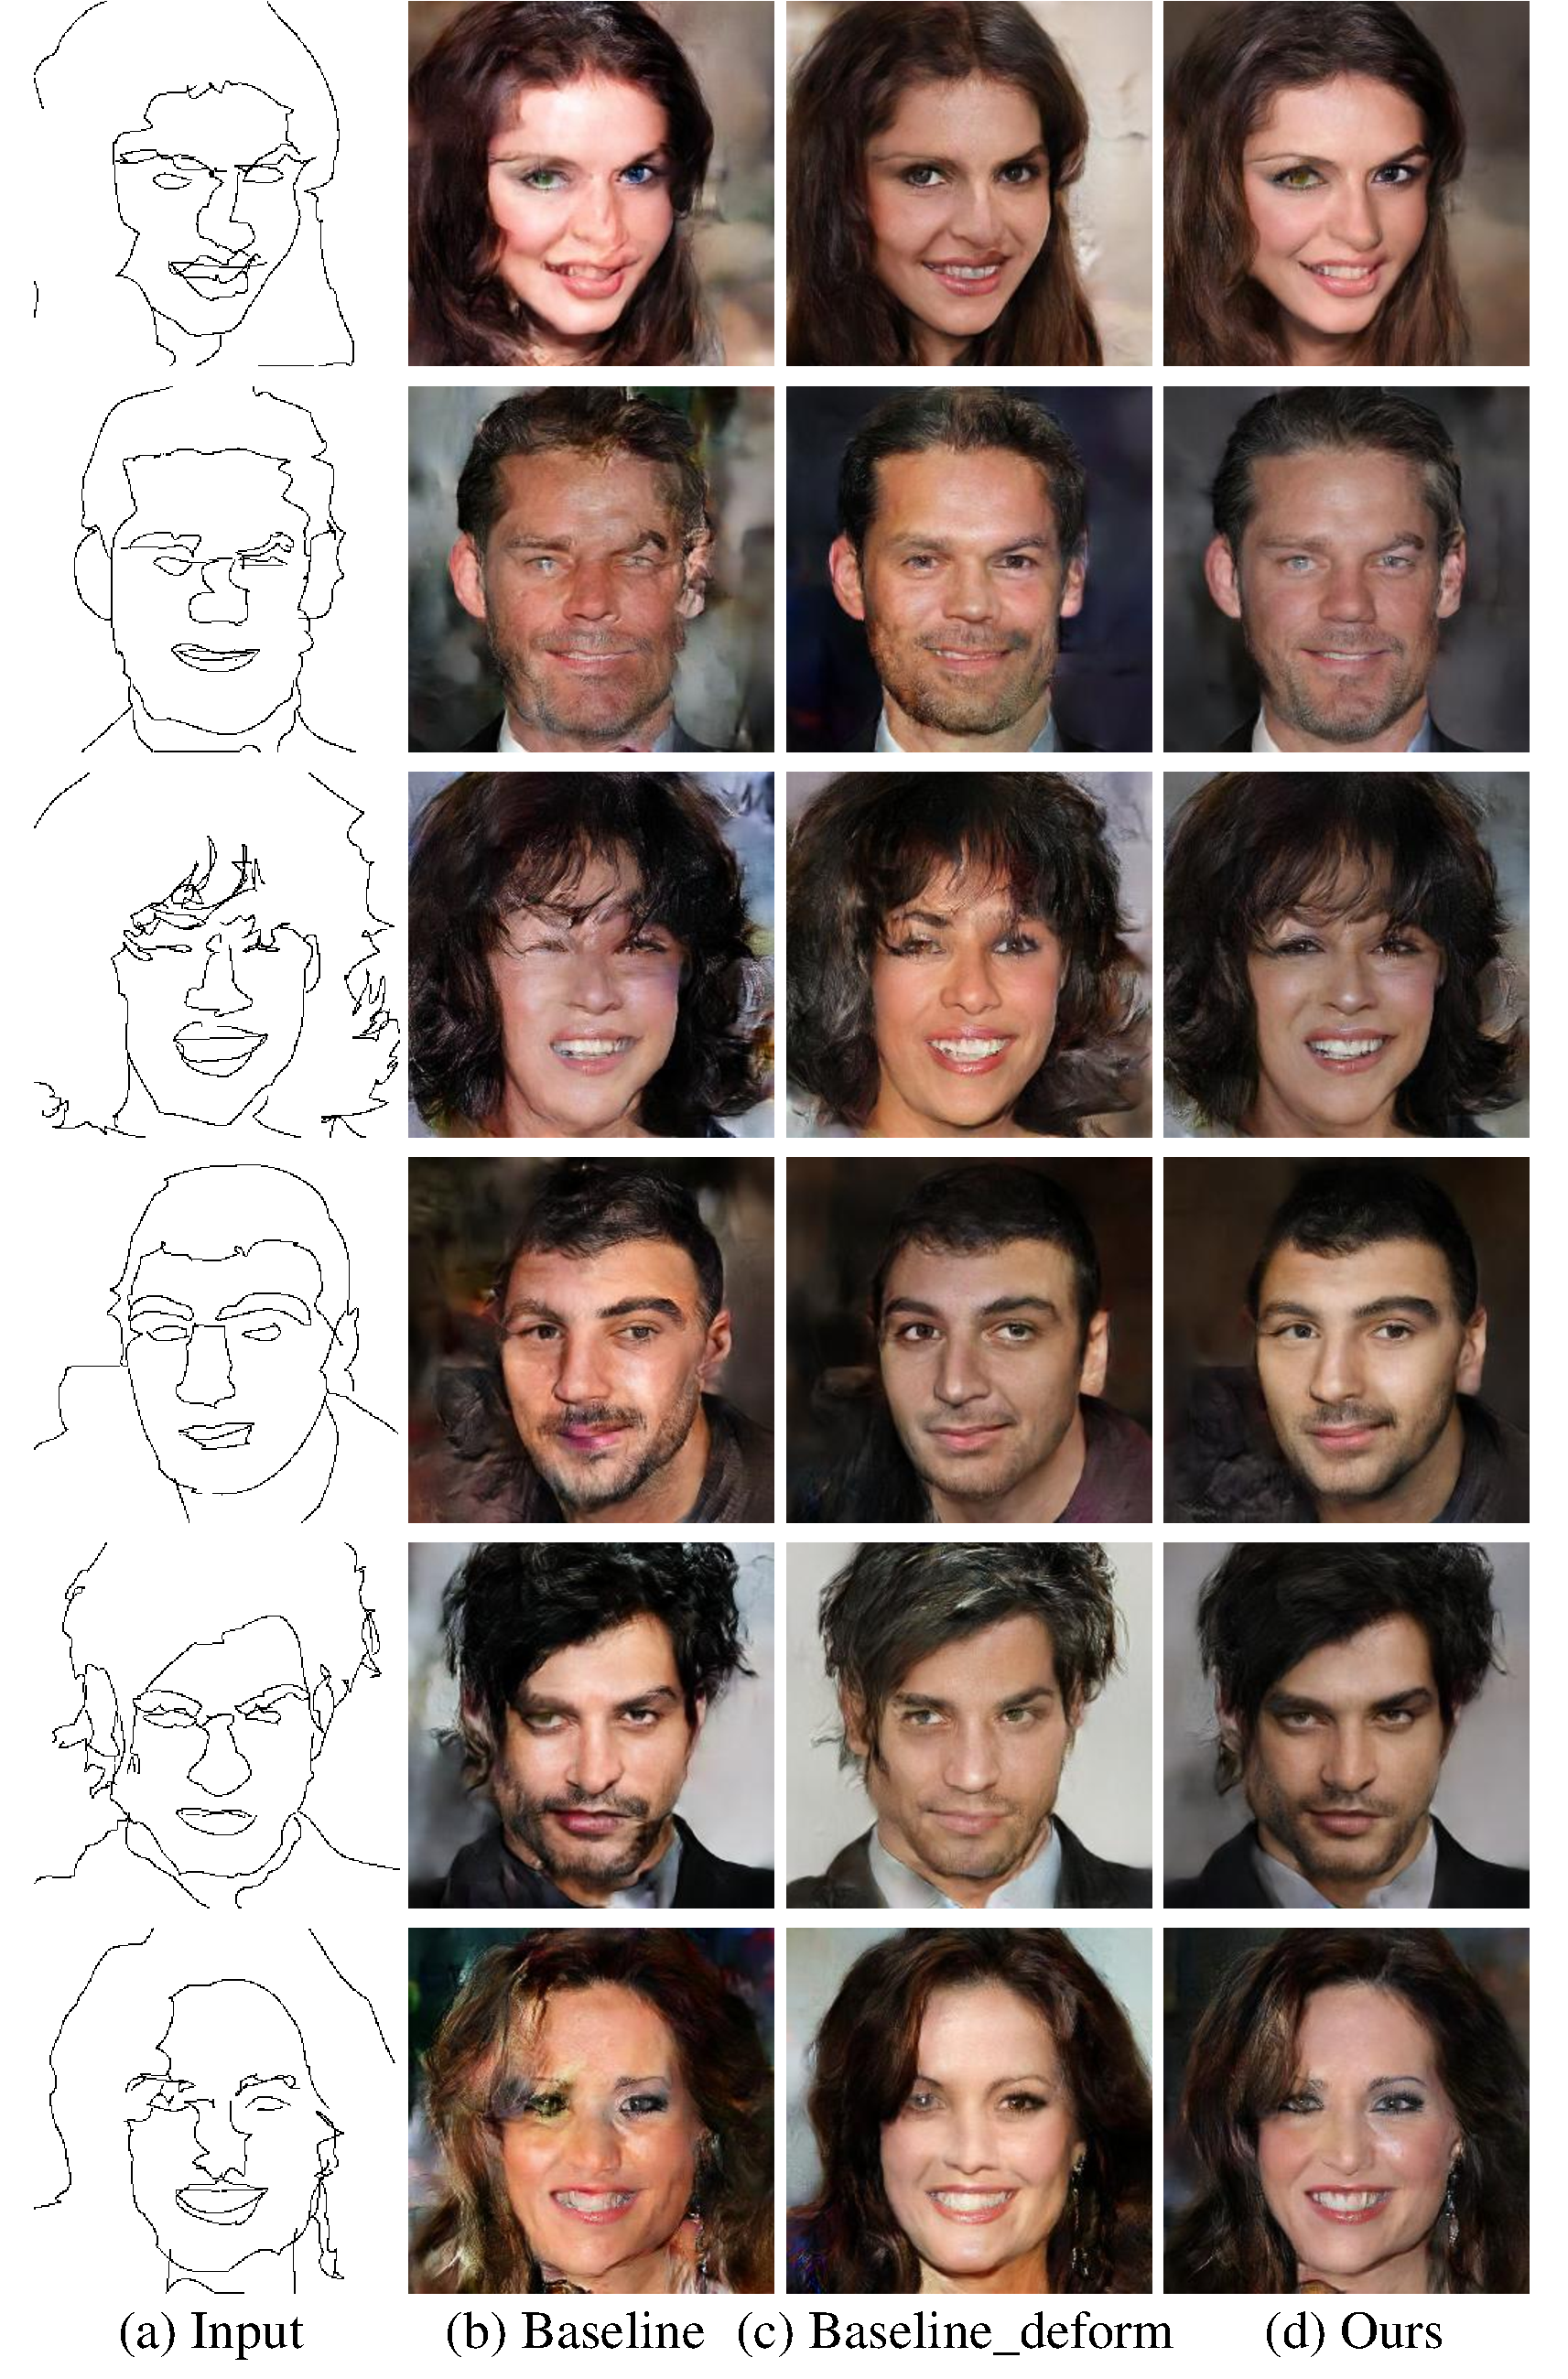
\includegraphics[width=0.9\linewidth]{figs/generalization_examples}
	\caption{\td{Result analyze, use generalization\_examples.pdf as placeholder}}
	\label{fig:generative_quality}
\end{figure}

\subsection{Comparison of Generalization Capability}

In order to verify the generalization ability of our model, we compare our model with state-of-the-art image translation models by testing with synthesized sketches of different levels of deformation, well-drawn sketches and poorly-drawn sketches by novel users.

\subsubsection{Different Level of Deformation}
As mentioned in Subsection~\ref{subsec:algorithm_data}, we deform an edge-aligned sketch $S$ to obtain a corresponding deformed sketch $S'$ by adding random offsets to the control points and end points of the vectorized strokes in $S$. 
The maximum offset $d$ is set to $11$ in the training data. 
We further create more deformed sketches with multiple levels of deformation, denoted as $S'_d$, by modifying the maximum offset $d$.
%
We examine the generalization ability of our model and baseline model on these deformed sketches. 
Note that the \textit{baseline} is trained with only edge-aligned sketches while our model and \textit{baseline\_deform} model are trained both edge-aligned sketches and deformed sketches with $d=11$.

In this experiment, the input sketches are deformed by larger offsets where the maximum $d$ is set to $30$. 
As shown in Figure~\ref{fig:generalization_examples}, strokes in sketches with larger deformation looks quite different from those in the training sketches including edge-aligned sketches $S$ and deformed sketches $S_{11}'$. 
%
\td{By adding deformed sketches into training data, \textit{baseline\_deform} produces better images than \textit{baseline}. However, when larger deformation occurs, \textit{baseline\_deform} suffers from artifacts in facial features, for example, the mouth in the first example, the eyes of the third and the last case in Figure~\ref{fig:generalization_examples}, 
In comparison, our model produces more realistic face images with more symmetric eyes and find textures, benefited from its ability of capturing shape feature from deformed strokes by our spatial attention pooling module. }
\begin{figure}
	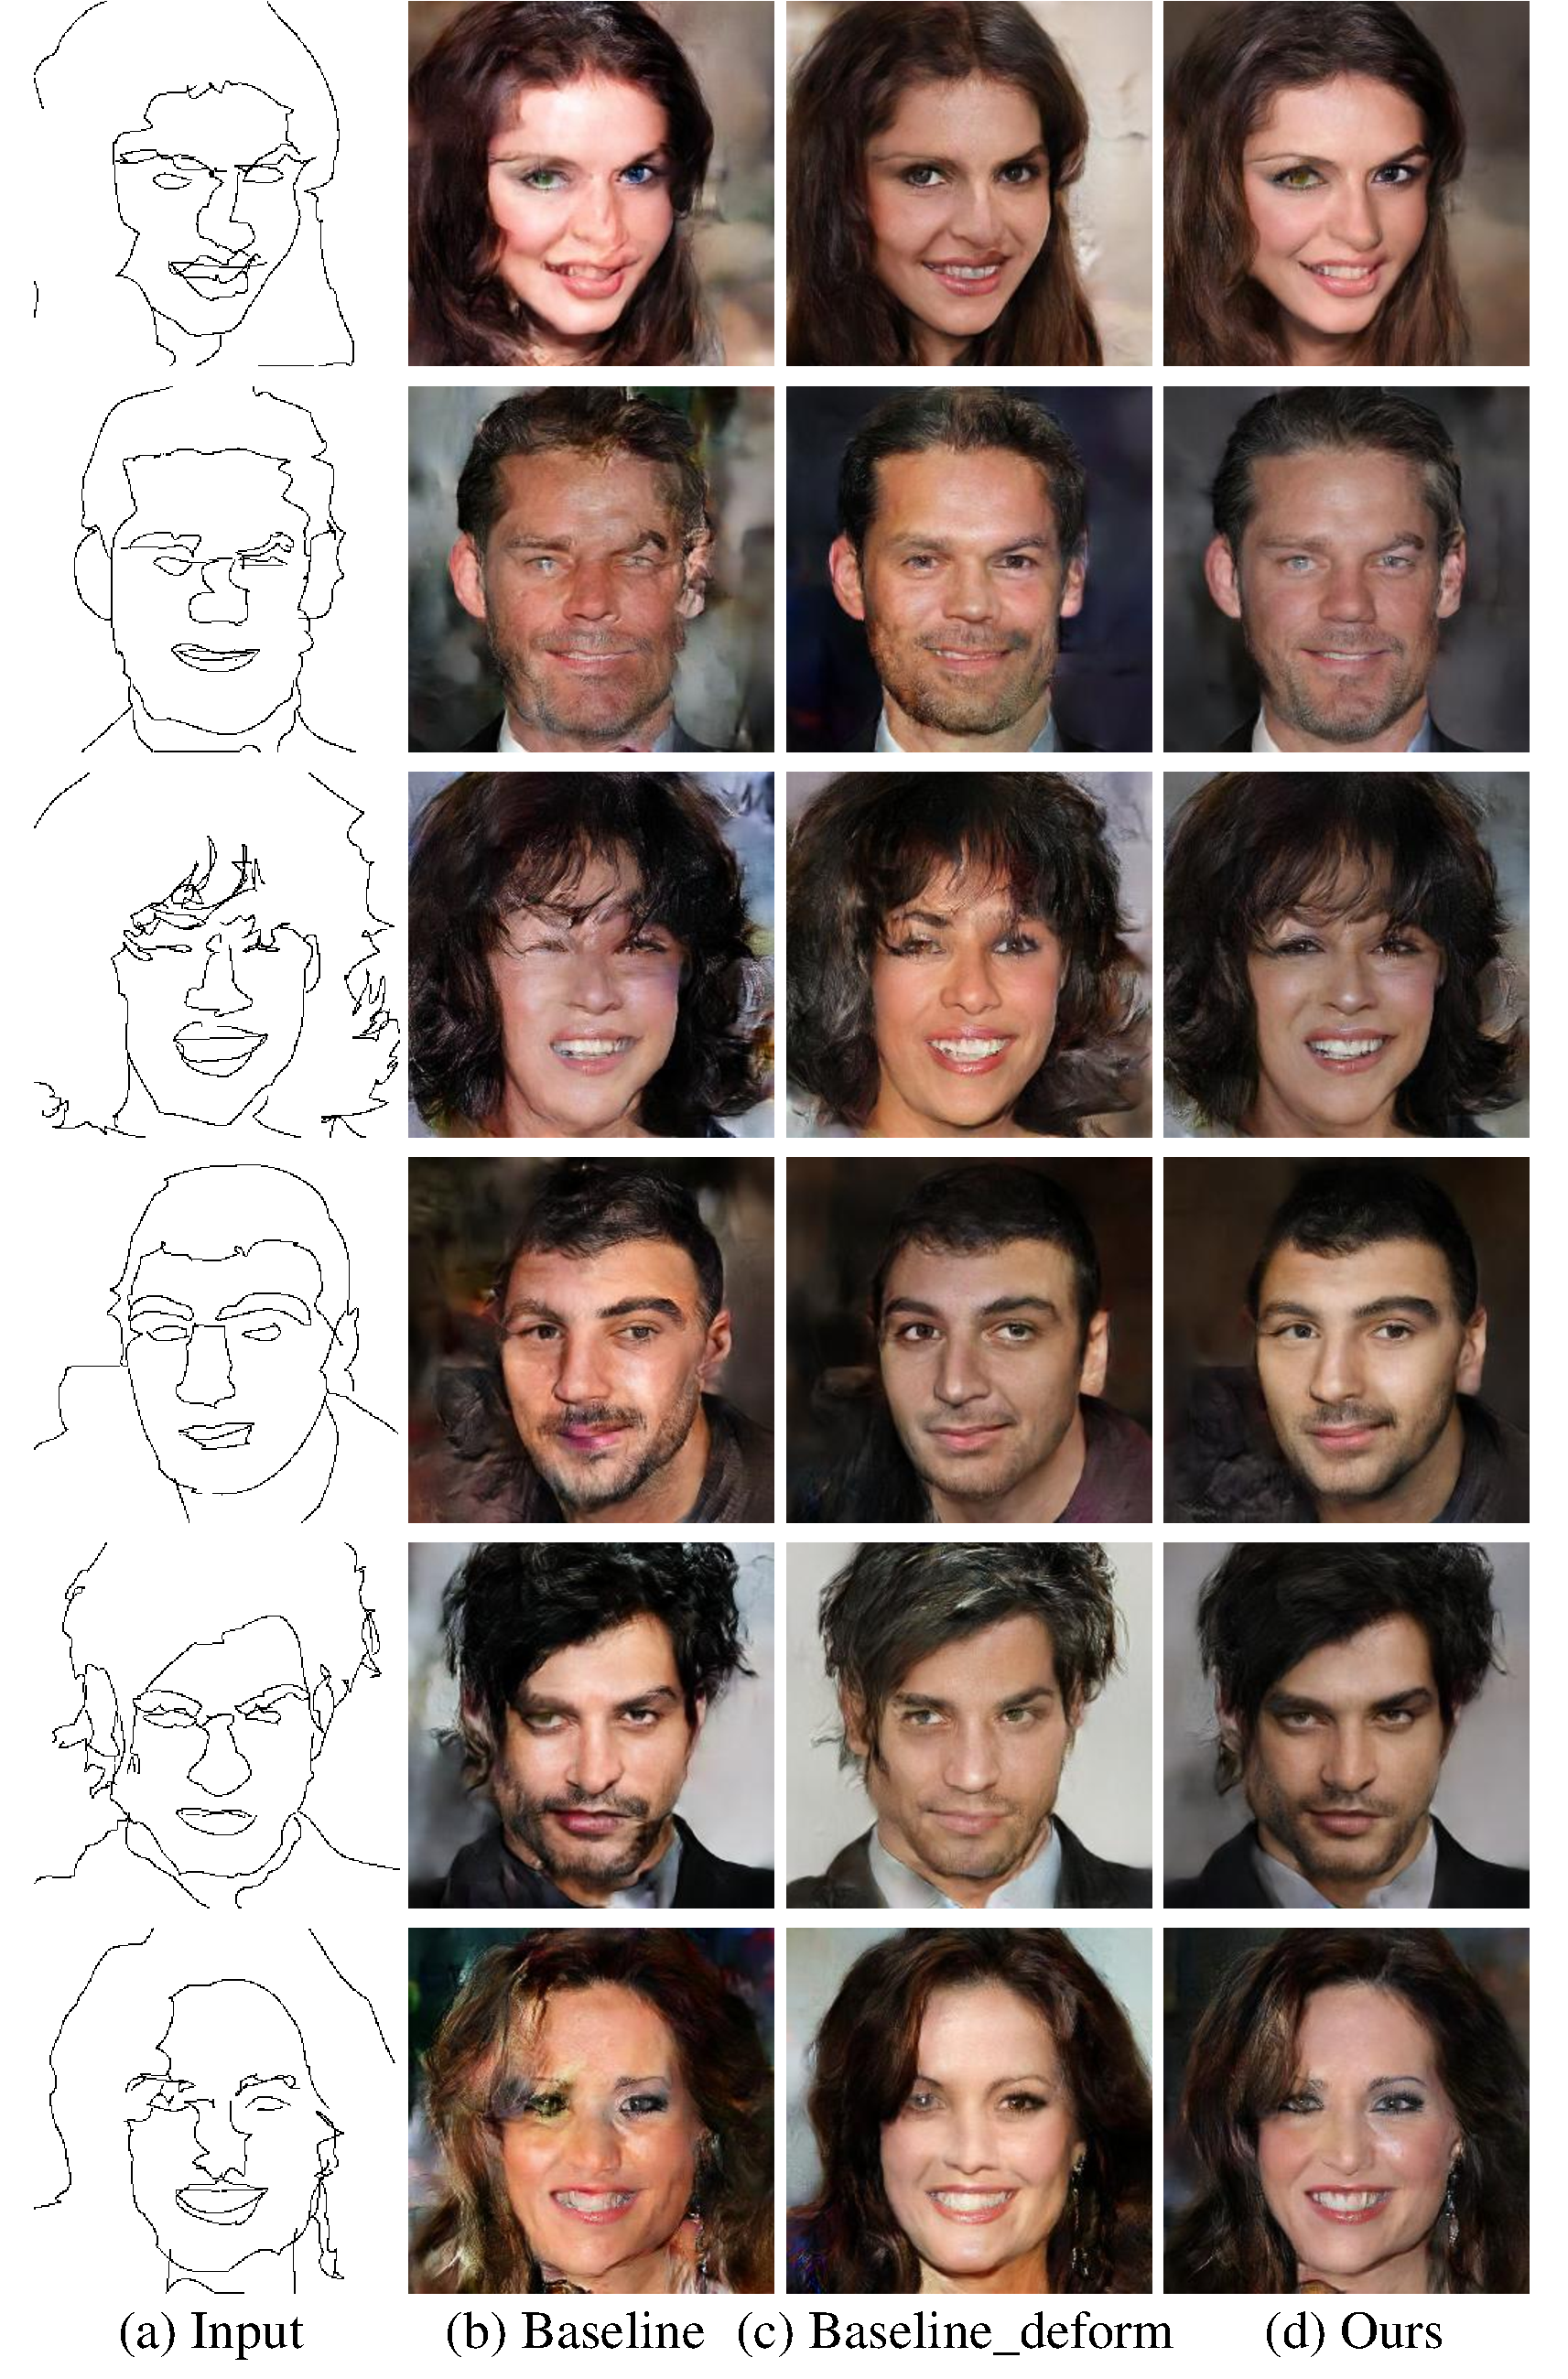
\includegraphics[width=0.9\linewidth]{figs/generalization_examples}
	\caption{\td{Result analyze}}
	\label{fig:generalization_examples}
\end{figure}

\subsubsection{Hand-Drawn Sketches}
Besides the synthesized sketches with stroke deformation, we further examine the model generalization ability by comparing performances of our model with baseline model tested with two kinds of hand-drawn sketches: expert-drawn sketches and common-user sketches drawn by users without professional painting skills.

\paragraph{Expert-Drawn Sketches}
We invite an expert with well-trained drawing skills to draw portrait sketches for testing. 
These expert sketches were drawn on a pen tablet so that the strokes are smooth and precise. 
Note that shading strokes are not drawn. 
%
Figure~\ref{fig:expert_sketches} shows a group of face images generated by different models from several expert-drawn sketches. 
%
Even with well-drawn strokes, the \textit{baseline} and \textit{baseline\_deform} frequently fail to produce realistic textures and complete structures of eyes or mouths. 
%
In comparison, our results are more realistic with fine textures and intact structures. 

\begin{figure}
	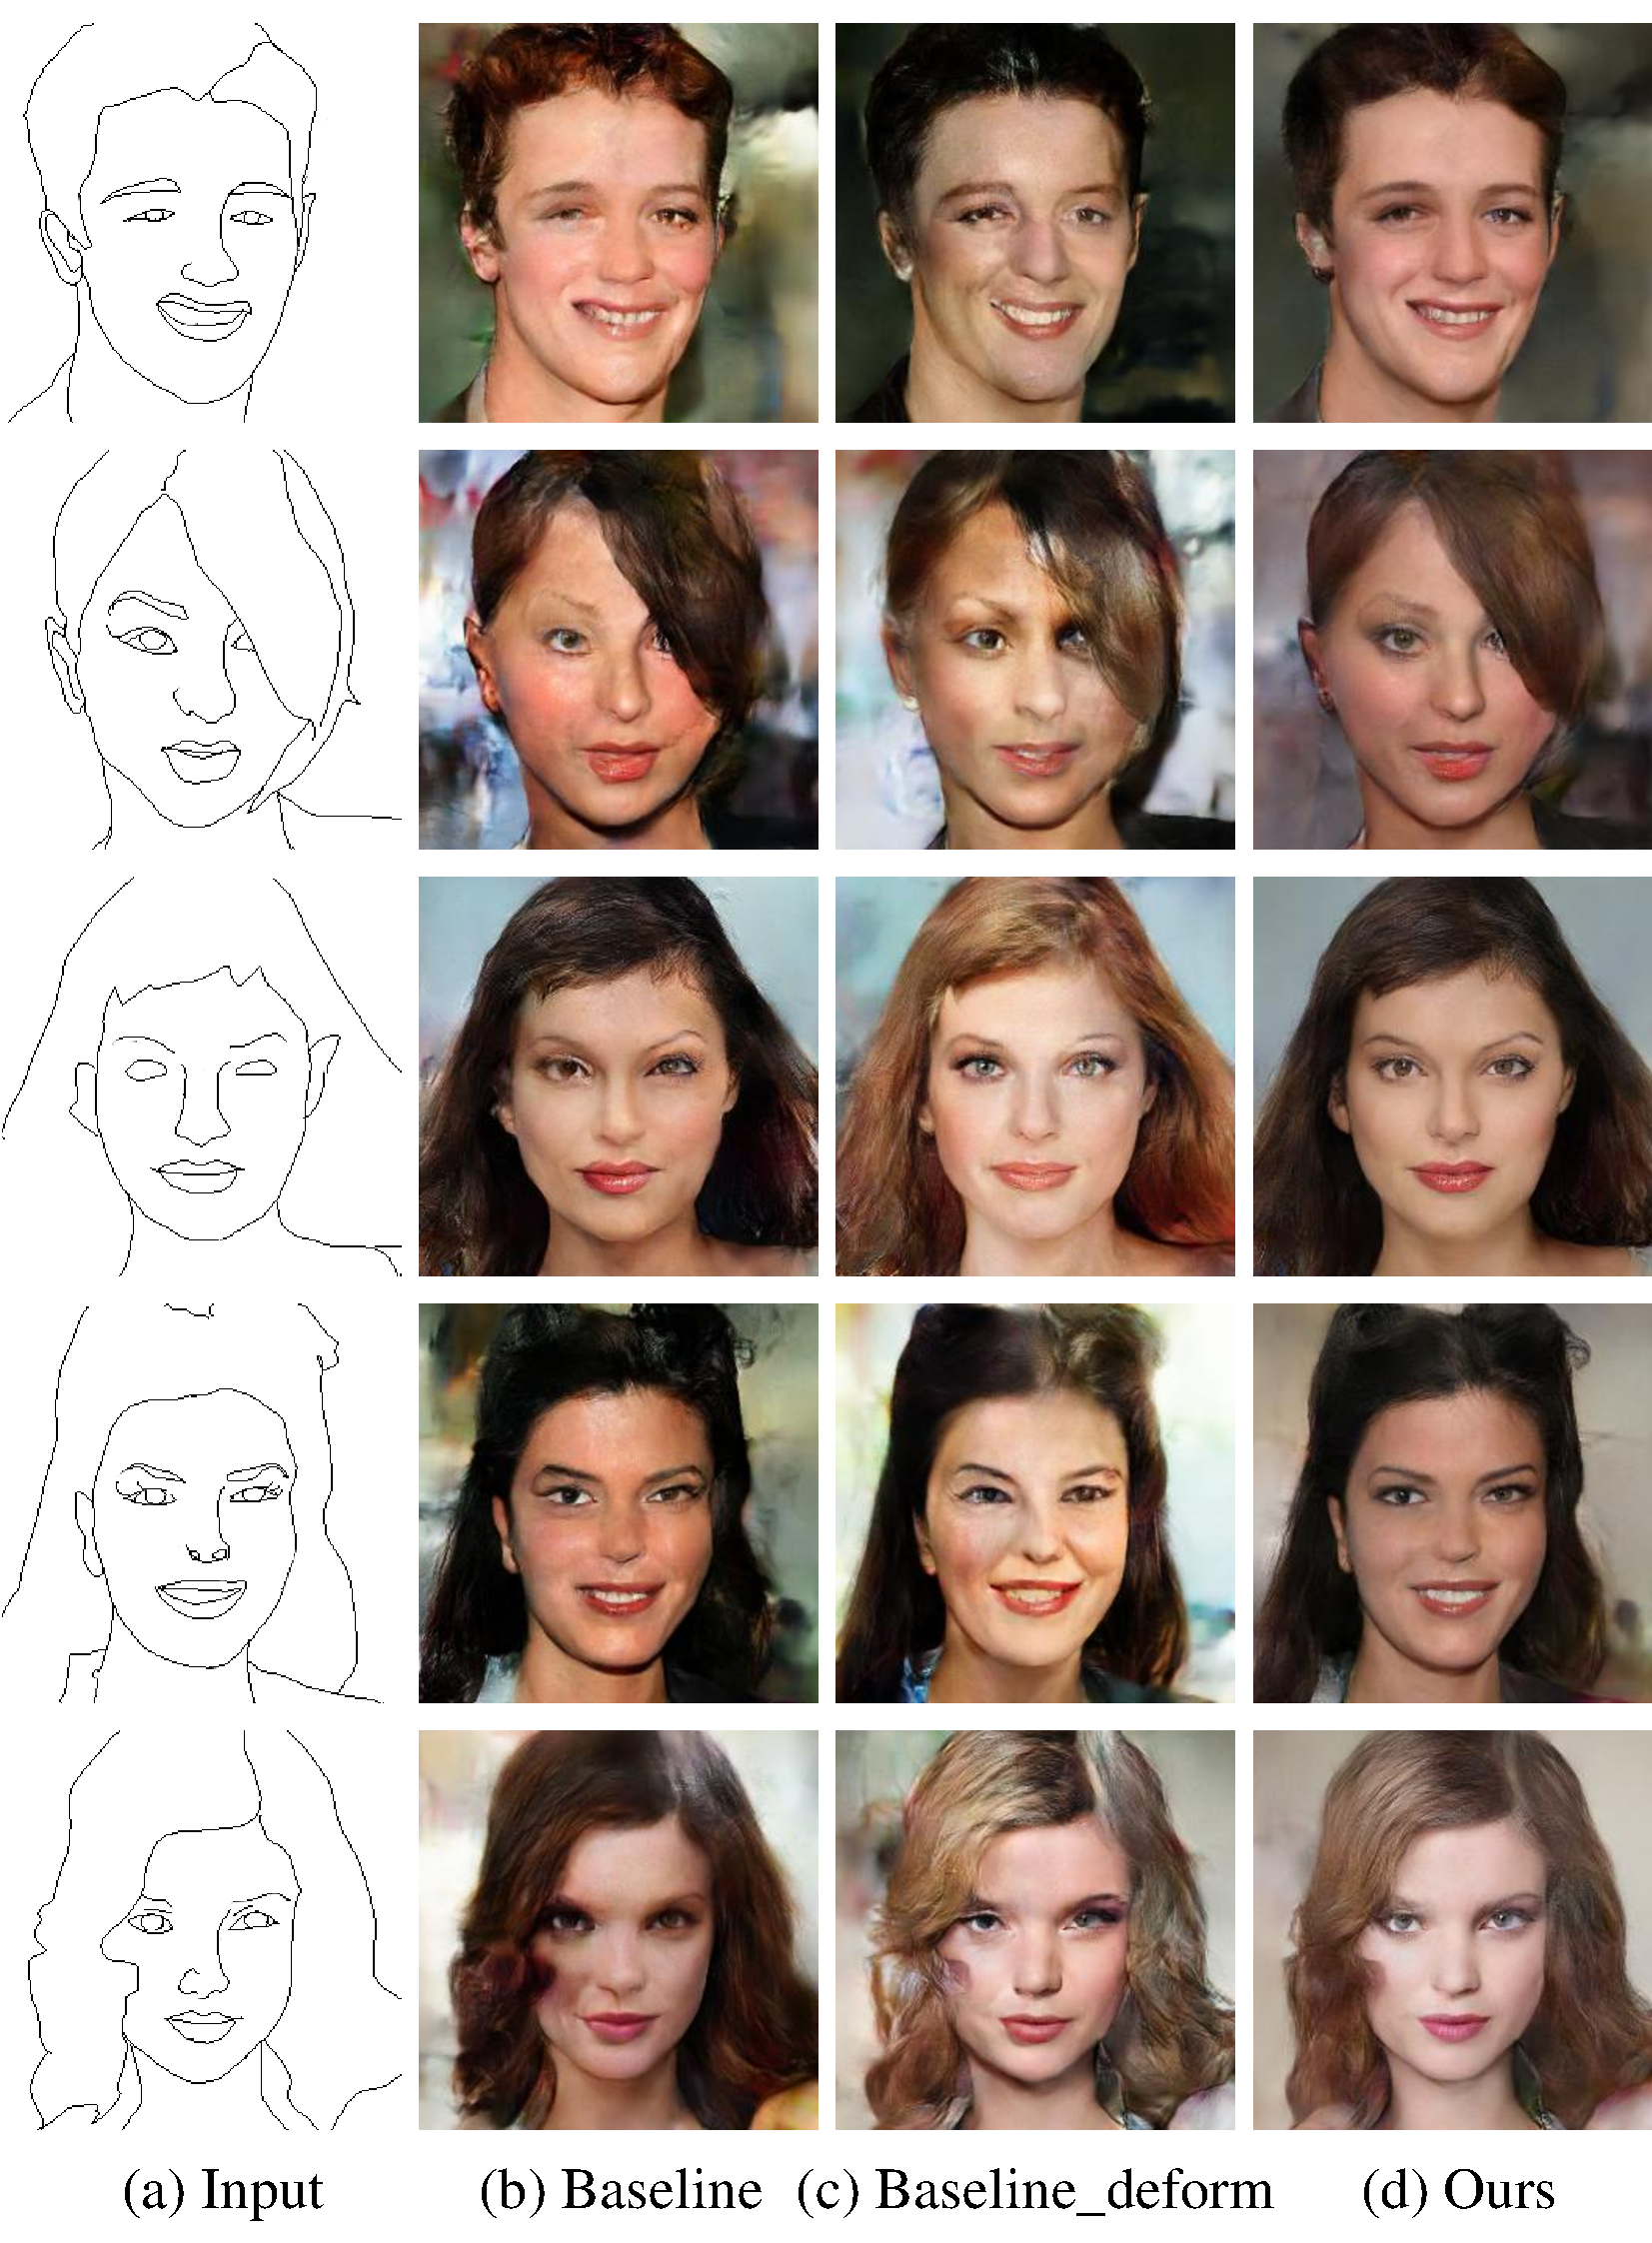
\includegraphics[width=0.9\linewidth]{figs/expertsketches}
	\caption{\td{Result analyze}}
	\label{fig:expert_sketches}
\end{figure}


\paragraph{Common Sketches}
We also invited a large number of graduate students without drawing skills to draw freehand sketches of their imagined faces using mouses. Hence, strokes of these common sketches rough depicts the desired face structure and shapes of facial features with some distortion. 
Moreover, common sketches turn to be of different levels of details. For example, some sketches contains many strokes inside the hair areas which are blank in the training sketches. 
%
Results shown in Figure~\ref{fig:common_sketches} demonstrate that our model is robust to these poorly-drawn sketches. 
In constrast, the diversity of stroke styles and detail levels significantly damage the quality of the results from the \textit{baseline} model and \textit{baseline\_deform} model.


\begin{figure}
	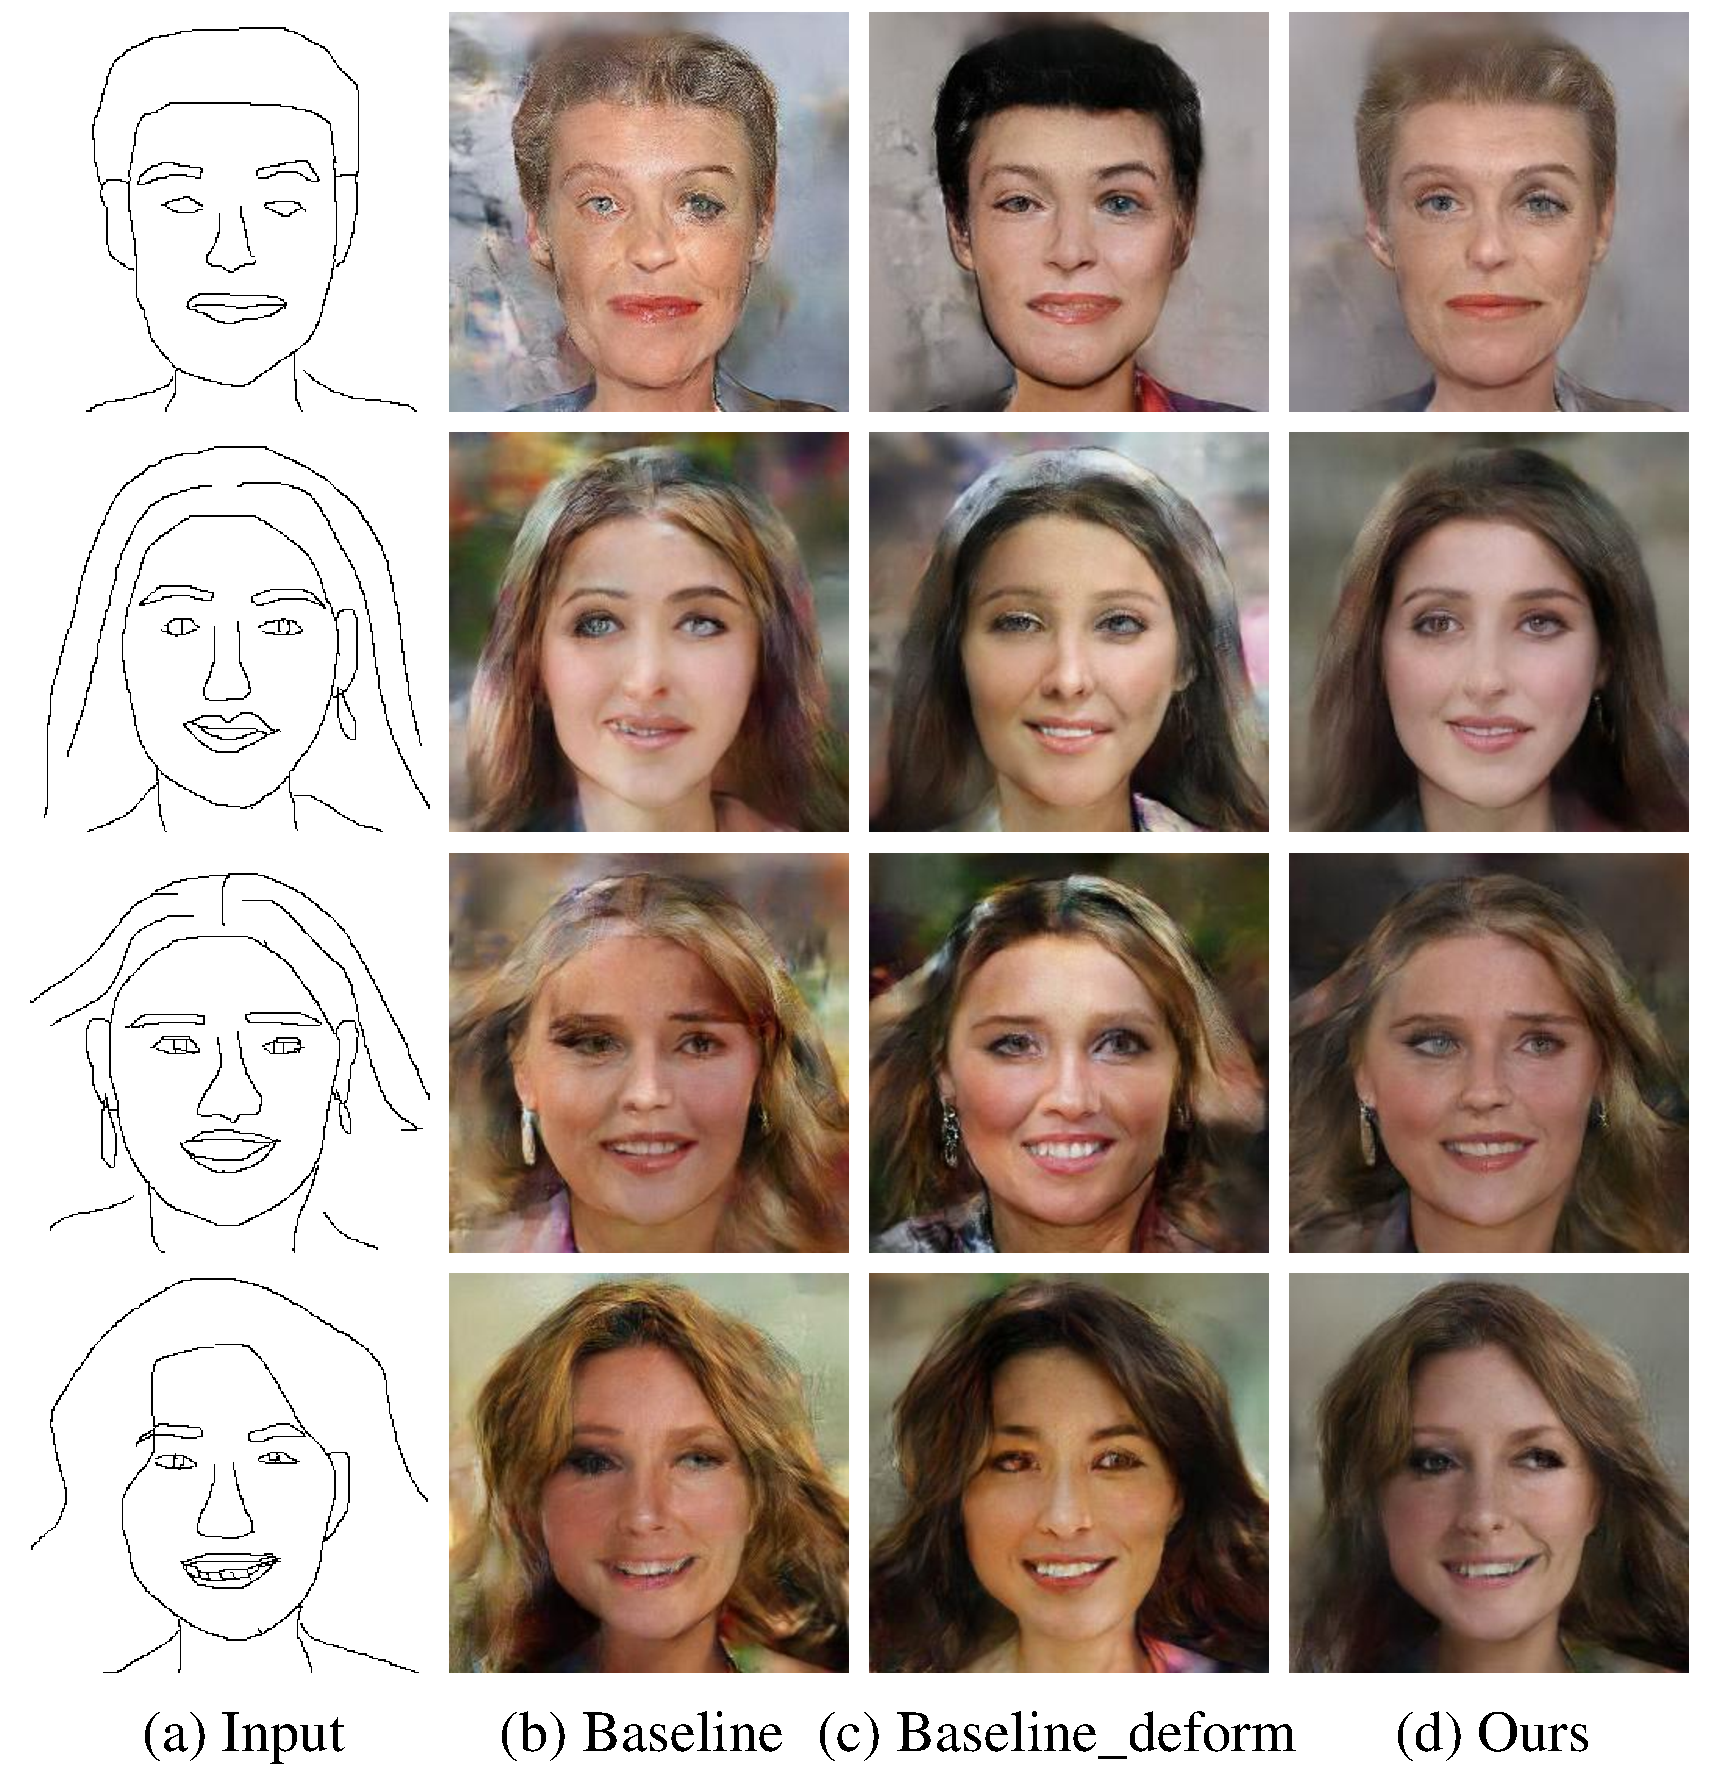
\includegraphics[width=0.9\linewidth]{figs/commonsketches}
	\caption{\td{Result analyze}}
	\label{fig:common_sketches}
\end{figure}


\subsection{Limitations and future work}




\section{Conclusion}
In this paper, we present DeepFacePencil, a novel deep neural network which allows common users to create photorealistic by freehand sketching.
%
The robustness of our sketch-based face generator comes from the proposed dual generators and the spatial attention pooling module. 
%
The proposed spatial attention pooling module adaptively adjusts the spatially varying balance between the image realism and the conformance between the input sketch and the synthesized image. 
%
By adding the SAP module to our dual-generator network and training the two generators simultaneously to enforce the main generator to effectively capture face structure and facial feature shapes from coarsely drawn sketches. 
Extensive experiments demonstrate that our DeepFacePencil successfully produce high quality face images from freehand sketches drawn by users in diverse drawing skills.
%



% Bibliography
\bibliographystyle{ACM-Reference-Format}
\balance 
\bibliography{sketch}
%\bibliography{sketchRef}



\end{document}
